\graphicspath{{chapters/ecm/}}
\chapter{ECM}

\section{ECM functional role}
The functional role of the extracellular matrix in tissue engineering involves providing a starting point for scaffold biodesign.
The ECM is a dynamic environment, which is produced and regulated by cells.
The ECM performs the following functions:

\begin{multicols}{2}
	\begin{itemize}
		\item aids in cell locomotion: cells in the body are in movement, mediated by the action of receptors (transmembrane proteins) and ligands into the ECM. The ECM should provide ligands for adhesion, which should be patterned in order to direct the cells in a specific place;
		\item transmits and distributes mechanical loads: the ECM, depending on the tissue and mechanical stimuli, should assume a specific structure in order to transmit the stress to the cells, without damaging the cells. Considering the scaffold design, this means that the mechanical properties of the scaffold are really important. The best mechanical properties to reproduce depend on the context;
		\item prevents premature mechanical failure;
		\item partitions cells and tissues into functional units;
		\item acts as a scaffold defining tissue and organ architecture;
		\item acts as a storage and dissipative device for elastic energy;
		\item acts as substrate for cell adhesion, growth, and differentiation: cell adhesion is really important, and should be provided even for cell growth and differentiation, because cells are adhesive dependant - especially cells for regeneration. This means that activation requires adhesion.
	\end{itemize}
\end{multicols}

\noindent
The ECM is a controlled complex network. It is formed by a complex network of proteins, glycoproteins and proteoglycans, which together provide tissue specific biophysical and biochemical properties. Remember that the ECM is tissue specific. The contact between the nucleus and the ECM is performed by integrins. We must find which genes should be activated for stimulating regeneration and the ligands for gene activation.
\\
\noindent
The ECM must interact with the cells. If the interaction is interrupted, the cells may go into pathology.
The ECM provides not only mechanical and structural support to cells and tissues, but also binds soluble ligands and transmembrane receptors to provide spatial coordination of signalling processes.
The ability of cells to sense the chemical, mechanical and topographical features of the ECM enables them to integrate complex, multiparametric information into a coherent response to the surrounding microenvironment.
Consequently, dysregulation or mutation of ECM components results in a broad range of pathological conditions.
\\
\noindent
The ECM is a composite material where cells sense the environment.
An example is a chondrocyte in a bone-like environment that will transform into bone, via calcification.
We need to pay attention to not having a damage effect instead of a therapeutic effect.
ECM polymers/network are instructive,  they provide structural and mechanical integrity to tissues.

\section{Components of the ECM}
\begin{itemize}
\item Physical signals are from fibronectin, vitronectin, collagen, laminin, fibrillin, GAGs, PG,...
\item Soluble signals: CF, cytokines, chemokines,...
\item Structure: composites, fiber-based, function dependent
\item Water: used to better tune mechanical properties. It can help the material to support the stress. Water is highly present in articular cartilage! The molecules able to ligate the water are GAGs and PGs. More water means more GAGs and PGs.
\item Mechano-transduction: translating mechanical stimuli
\end{itemize}
\noindent
Fibers are made of collagen, which can form fibrils (very elastic structures), fiber (a little bit thicker) or bundle (composition of more fibers all together). In addition, to better tune the mechanical properties without changing the chemistry, nature can also change the organisation of the fibers: they can be well oriented or randomly distributed, depending on the mechanical stimuli and the direction of them.
\\
\\
\noindent
Signals are important for the adhesion, so other molecules are introduced into the scaffold as well, adhesion ligands and collagen (to form the structure, it is able to provide ligand too).
Another strategy is trying to reduce the number of the elements, in particular the number of the molecules produced by the cells. How? By designing multi-functional polymers, one polymer must do many things. Finally, it is possible to employ soluble signals. Cells can communicate with each other - very distant cells communicate thanks to soluble signals.
\\
\\
\noindent
Thanks to the cross-talk between cells and ECM we have the trigger and the control of many processes. ECM/cells crosstalks facilitate and regulate: pattern formation, morphogenesis, cell fate, daily cellular processes, wound healing, tissue homeostasis.

\subsection{Stem cells}
The environment is important even for stem cells. Stem cells are rare cells that are uniquely capable of both reproducing themselves (self-renewing) and generating the differentiated cell types that are needed to carry out specialised functions in the body.
This is important in the embryogenesis and a balanced control between self-renewed cells and differentiation is fundamental in the healing process and homeostasis. If it is deregulated we can have tumorigenesis, degeneration, pathology,...
Pay attention: the scaffold sends information, we can induce cancer formation too!
Changing the organization of the fibers in the ECM leads to modifications in water content and rigidity ; as a result, we will end up with a completely different signal.

\section{The matrixome: chemistry of the ECM}
\begin{figure}[ht]
\centering
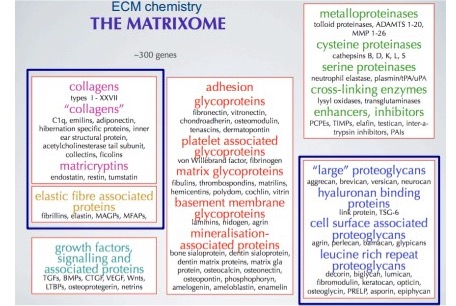
\includegraphics[width=0.8\textwidth]{matrixome}
\caption{\label{fig:matrixome}}
\end{figure}

\noindent
The stiffness is controlled by collagens, elasticity by elastic fibers.
Signalling molecules are used for cell-cell communications e.g. growth factors.
Adhesion molecules promote cell adhesion, pattern to drive the mobility direction.
The proteinases are important to destroy the proteins we don’t want, they provide dynamicity. The GAGs and PGs are relevant for the water content of the ECM.
Something important for scaffold design is that we can use proteinase to degrade the scaffold once we need to degrade it, not before.
\\
\noindent
Matricellular proteins are extracellular modulators of cell function expressed at high level during development and in response to injury. They are modulators of cell matrix interactions and bind to many cell surface receptors, the ECM, GFs, cytokines and proteases. Their role is to induce de-adhesion in contrast to the adhesivity of most matrix proteins (migration).
\noindent
Functions:
\begin{itemize}
\item cell adhesion, migration, chemotaxis
\item matrix assembly and collagen fibrillogenesis
\item regulation proliferation/apoptosis
\item binding/activation GFs and cytokines
\item angiogenesis and tumour growth
\end{itemize}

%Example: support of a state of intermediate adhesion (disruption of focal adhesion and reorganisation of actin stress fibers):	TSP1 and 2, Tenascin-C, SPARC
%Cercare più info/appunti

\section{Collagen}
Collagen is one of the most important proteins for the ECM, as it provides structural properties. Collagen is produced by cells: the production starts in the cytoplasm,  while the final assembly is performed outside the cell.
Fibrils are formed first, then assembled into fibers and bundles.
\noindent
How can collagen build the network?
\begin{itemize}
\item connective tissue: less density, soft network, more water, fiber and fibrils
\item meniscus: parallel fibers, more density, packed fibers, because of different functions, bundle (more stress)
\item myocardium: mechanical stresses, it should support the growth in one direction
\end{itemize}
\noindent
Cells can migrate in this low porosity material through a specific enzymatic process,  which allows the space to be opened up.
Collagen is non-homogeneous, bottom-up, multi-functional, dynamic and has a hierarchical structure. The structure is function dependent.
We have three chains,  which can reach a helix formation (quaternary structure). If we increase the chemical bridges between the helices we control elasticity.
\\
\\
\noindent
The ECM is degraded by cell-secreted proteases (remodelling) and releasing of bioactive component.
Natural ECMs modulate tissue dynamics through their ability to locally bind, store and release soluble bioactive ECM effectors such as GFs.
Our scaffold should promote cell migration.
\\
\\
\noindent
Collagen is a family of proteins, we have at least 23 different types of collagens. Depending on the tissue, we have the prevalence of one type on another type. In the cartilage for example we have collagen type II. In tendons we have type III collagen, which is really similar to jellyfish collagen, currently commercialized.

\section{Fibronectin}
Fibronectin is a large matrix glycoprotein present in most body tissues fluids.
Functionally, it is the classic example of an adhesive glycoprotein, binding and interconnecting extracellular matrix components with each other and to the surface of the cells.
It is one of the most important molecules through which cells interact with the surrounding environment.
The binding of fibronectin to the cell surface’s integrin receptors plays a critical role in the cell migration (during the development and postnatally).
\\
\\
\noindent
Fibronectin is made of two identical chains connected by a disulphide bond, a dimer.
We can recognise different sections:
\begin{itemize}
\item one can interact with fibrin and heparin
\item one can interact with gelatine and collagen
\item one can interact with the cell receptor (arg-gly-asp ac. sequence)
\item one can interact with polysaccharide heparin
\item one can interact with fibrin
\end{itemize}
\noindent
These molecules must be able to interact and crosslink because in this way if we have a stimulus that acts in the collagen, for example, the other parts of the ECM can sense said stimulus. In addition, many regions of the ECM are able to interact with cells, controlling the structure and cellular activity.
\\
\\
\noindent
In ECM we have fibronectins, collagen, gel-forming polysaccharides, water, actin and the cell (figure \ref{fig:structure}).
The transmembrane can sense what is going on in the external side and transfer the information to the internal part and eventually to the nucleus to activate a specific gene expression.
The interactions are important and interesting, the scaffold needs to provide the ability to interact with the same exact mechanism and cells must work in an appropriate way.
We don’t want dysregulation of the mechanisms and the tissue, so we need the natural mechanism of interaction.

\begin{figure}[ht]
\centering
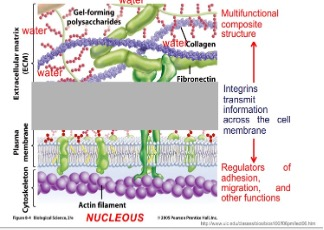
\includegraphics[width=0.6\textwidth]{structure}
\caption{\label{fig:structure}}
\end{figure}

\noindent
The ECM is a mosaic structure, a guide for cell functions.
Should the scaffold replicate the ECM? Partially, yes, but especially the functions! 
Large molecules are difficult to manage, maybe using a smaller molecule (nectin instead of fibronectin) is easier.
Fibronectin is needed to reproduce the complete ECM, but nectin is sufficient to promote cell growth.

\subsection{Fibronectin multifunctionality}
The RGD-loop is strategically placed to undergo strong conformational changes and constitutes a mechanosensitive switch for recognition by integrin receptors.
Depending on the mechanical stimulus, fibronectin can assume specific conformations, changing its activity.

\section{Proteoglycans and GAGs}

\textbf{Proteoglycan}: head core protein + chain of polysaccharides (GAGs), which is hydrophilic (figure \ref{fig:pgag}). 
Proteoglycans are responsible for controlling the water content of the tissue and are especially important in case of mechanical stresses.
Many proteoglycans can be linked together via long hyaluronic acid chains, forming giant com- plexes. 
Because of their negative charges, glycosaminoglycans and proteoglycans together control the $H_2O$ content of the tissue, determining the degree of ”squishiness” of the matrix. 
They also allow for $H_2O$ reentry after tissue compression: in this situation water gets squeezed out and the negative charges of different molecules draw near. 
This generates an electrical repulsion that summons water from the peripheries.
\\
\\
\noindent
\textbf{Glycosaminoglycans} (GAGs) are linked to the core proteins, we can have:
\begin{itemize}
\item hyaluronic acid
\item chondroitin sulfate
\item keratan sulfate
\end{itemize}
\noindent
GAGs are long linear polysaccharides consisting of repeating disaccharide units (i.e. two-sugar units). 
The repeating two-sugar unit consists of a uronic sugar and an amino sugar, which is usually sulfated. 
\\
\\
\noindent
In proteoglycans, the big protein is able to interact with water and the core protein, hydrophobic, is covered by hydrophilic molecules.
The water should be able to go out when the tissue undergoes mechanical stress to ensure homeostasis.
This is a reversible mechanism,  the scaffold must have specific properties to resist stress and control water flow.
\begin{figure}[ht]
\centering
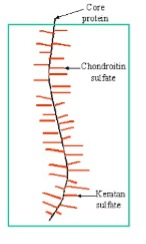
\includegraphics[width=0.3\textwidth]{pgag}
\caption{\label{fig:pgag}}
\end{figure}

\section{Modelling nature}
Our goal is to stimulate the cell.
The environment is dynamic, and the interactions are possible thanks to the water.
The interactions between cells and environment are relevant to regulate a lot of processes, from cell fate to tissue formation and regeneration.
Our scaffold will be one of the components that will collaborate to regenerate the tissue.
Once again, we need a model, which is nature.
We need to leave cells work in a natural way.
Living organisms naturally provide a multiplicity of materials, architectures, systems and functions, all resulting in from stringent selection process (evolution).
\noindent
Strategy:
\begin{itemize}
\item polymers (materials) able to integrate
\item molecular synthesis (by cells) at very high level of organisation (molecular recognition, multifunctionality, self-diagnostic, destruction-recycling, bottom-up approach)
\item structure (self-assembling, molecule interactions, interfaces, etc) dynamics
(responsive polymers, adaptation, self-healing)
\end{itemize}
\noindent
The bottom-up approach is more bio-mimetic,  as it reflects how nature works [self-assembling blocks, proteins are formed automatically from amino acids].
We should also focus our attention on building a context-specific microenvironment.
\\
\\
\noindent
Apoptosis is a programmed cell death, in which cells are encapsulated by vesicles and removed.
Necrosis instead happens when the cellular membrane is damaged, we have inflammation.
During necrosis the activity of macrophages is increased, producing also inflammation for neighbouring cells.
It has been suggested to induce tumour cell death through apoptosis to avoid upregulating inflammation.
